% =====================================================================
%  Introduction to Neuroscience — Sessions 10-12: Activity booklet (The relay)
%  Companion to NEUR_S10_12_relay. Page numbers are referred to on
%  the slides; keep the \newpage breaks. Relay Lab link: \lablink below.
% =====================================================================
\documentclass[12pt,a4paper]{article}
\usepackage[margin=1.9cm,bottom=2.2cm]{geometry}
\usepackage[T1]{fontenc}
\usepackage{helvet}
\renewcommand{\familydefault}{\sfdefault}
\usepackage{setspace}
\setstretch{1.18}
\usepackage{ragged2e}
\usepackage{enumitem}
\usepackage{array}
\usepackage{booktabs}
\usepackage{xcolor}
\usepackage{amssymb}
\usepackage{tikz}
\usetikzlibrary{arrows.meta}
\usepackage{tcolorbox}
\tcbuselibrary{skins}
\usepackage{fancyhdr}
\usepackage{textcomp}
\usepackage{pgfplots}
\pgfplotsset{compat=1.17}
\usepackage{qrcode}
\usepackage{url}
\urlstyle{sf}

\newcommand{\sessnum}{10--12}  % change here if the session is renumbered
\definecolor{kprimary}{HTML}{1F3A5F}
\definecolor{kaccent}{HTML}{B85A0E}
\definecolor{kgreen}{HTML}{23665A}
\definecolor{kred}{HTML}{A12F24}
\definecolor{kpale}{HTML}{F7F3EA}
\definecolor{kgrey}{HTML}{4B5563}

\pagestyle{fancy}\fancyhf{}
\renewcommand{\headrulewidth}{0pt}
\fancyfoot[L]{\small\color{kgrey}Introduction to Neuroscience \,$\cdot$\, Sessions \sessnum\ activity booklet}
\fancyfoot[R]{\small\bfseries\color{kprimary}Page \thepage}
\setlength{\parindent}{0pt}
\setlength{\parskip}{4pt}
\hyphenpenalty=10000 \exhyphenpenalty=10000 \tolerance=9000 \emergencystretch=3em
\RaggedRight
\setlist{itemsep=3pt,topsep=4pt}

\newcommand{\pagehead}[1]{{\color{kprimary}\LARGE\bfseries #1}\par\vspace{2pt}{\color{kaccent}\rule{\linewidth}{1.2pt}}\par\vspace{4pt}}
\newcommand{\infopill}[2]{{\setlength{\fboxsep}{4pt}\fcolorbox{kaccent}{kaccent!8}{\textbf{#1:}\ #2}}}
\newcommand{\actinfo}[3]{\infopill{Time}{#1}\hspace{0.5em}\infopill{Who}{#2}\hspace{0.5em}\infopill{You need}{#3}\par\medskip}
\newcommand{\lines}[1]{\par\foreach \i in {1,...,#1}{\vspace{0.75cm}\hrule height 0.4pt}\par\medskip}
\newcommand{\blank}[1][3.2cm]{\rule{#1}{0.4pt}}
\newcommand{\cb}{$\square$\ }
\newtcolorbox{stepsbox}[1][]{enhanced,colback=kpale,colframe=kprimary,arc=2mm,boxrule=0.8pt,left=8pt,right=8pt,top=5pt,bottom=5pt,
  halign=flush left,title={\bfseries Steps (tick each one when done)},fonttitle=\normalsize,coltitle=white,#1}
\newtcolorbox{infobox}[1][]{enhanced,colback=kprimary!4,colframe=kprimary!70,arc=2mm,boxrule=0.6pt,left=8pt,right=8pt,top=4pt,bottom=4pt,
  halign=flush left,fonttitle=\normalsize\bfseries,coltitle=white,#1}
\newtcolorbox{studycard}[1][]{enhanced,colback=white,colframe=kgreen,arc=2mm,boxrule=0.8pt,left=7pt,right=7pt,top=3pt,bottom=3pt,
  halign=flush left,fonttitle=\normalsize\bfseries,coltitle=white,#1}


% ---------- at-a-glance additions (v2), same as the deck ----------
\definecolor{cNa}{HTML}{B85A0E}
\definecolor{cK}{HTML}{6A3D9A}
\definecolor{cCl}{HTML}{23665A}
\definecolor{cCa}{HTML}{A12F24}
\newcommand{\Na}{\textcolor{cNa}{\textbf{Na$^{+}$}}}
\newcommand{\K}{\textcolor{cK}{\textbf{K$^{+}$}}}
\tikzset{
  ionNa/.style={circle,fill=cNa,text=white,font=\footnotesize\bfseries,inner sep=0pt,minimum size=0.62cm},
  ionK/.style={circle,fill=cK,text=white,font=\footnotesize\bfseries,inner sep=0pt,minimum size=0.62cm},
  nb/.style={circle,fill=kprimary,text=white,font=\small\bfseries,inner sep=0pt,minimum size=0.55cm}}

\tikzset{badge/.style={circle,fill=kprimary,text=white,font=\scriptsize\bfseries,inner sep=0pt,minimum size=0.42cm}}
% ---- traces from the Relay Lab models (Part 2: integrate-and-fire neuron; Part 3: receptor kinetics) ----
\newcommand{\lifA}{(0.00,-65.00) (0.20,-65.00) (0.40,-65.00) (0.60,-65.00) (0.80,-65.00) (1.00,-65.00) (1.20,-65.00) (1.40,-65.00) (1.60,-65.00) (1.80,-65.00) (2.00,-65.00) (2.20,-65.00) (2.40,-65.00) (2.60,-65.00) (2.80,-65.00) (3.00,-65.00) (3.20,-65.00) (3.40,-65.00) (3.60,-65.00) (3.80,-65.00) (4.00,-65.00) (4.20,-65.00) (4.40,-65.00) (4.60,-65.00) (4.80,-65.00) (5.00,-64.92) (5.20,-64.19) (5.40,-63.51) (5.60,-62.90) (5.80,-62.34) (6.00,-61.84) (6.20,-61.37) (6.40,-60.95) (6.60,-60.57) (6.80,-60.23) (7.00,-59.92) (7.20,-59.63) (7.40,-59.38) (7.60,-59.15) (7.80,-58.94) (8.00,-58.76) (8.20,-58.60) (8.40,-58.45) (8.60,-58.33) (8.80,-58.22) (9.00,-58.12) (9.20,-58.04) (9.40,-57.97) (9.60,-57.91) (9.80,-57.86) (10.00,-57.82) (10.20,-57.79) (10.40,-57.77) (10.60,-57.76) (10.80,-57.75) (11.00,-57.75) (11.20,-57.76) (11.40,-57.78) (11.60,-57.79) (11.80,-57.82) (12.00,-57.84) (12.20,-57.87) (12.40,-57.91) (12.60,-57.95) (12.80,-57.99) (13.00,-58.03) (13.20,-58.08) (13.40,-58.13) (13.60,-58.18) (13.80,-58.23) (14.00,-58.29) (14.20,-58.34) (14.40,-58.40) (14.60,-58.46) (14.80,-58.52) (15.00,-58.58) (15.20,-58.64) (15.40,-58.70) (15.60,-58.77) (15.80,-58.83) (16.00,-58.89) (16.20,-58.96) (16.40,-59.02) (16.60,-59.09) (16.80,-59.15) (17.00,-59.22) (17.20,-59.28) (17.40,-59.34) (17.60,-59.41) (17.80,-59.47) (18.00,-59.54) (18.20,-59.60) (18.40,-59.66) (18.60,-59.73) (18.80,-59.79) (19.00,-59.85) (19.20,-59.91) (19.40,-59.97) (19.60,-60.04) (19.80,-60.10) (20.00,-60.16) (20.20,-60.22) (20.40,-60.27) (20.60,-60.33) (20.80,-60.39) (21.00,-60.45) (21.20,-60.51) (21.40,-60.56) (21.60,-60.62) (21.80,-60.67) (22.00,-60.73) (22.20,-60.78) (22.40,-60.84) (22.60,-60.89) (22.80,-60.94) (23.00,-60.99) (23.20,-61.05) (23.40,-61.10) (23.60,-61.15) (23.80,-61.20) (24.00,-61.25) (24.20,-61.29) (24.40,-61.34) (24.60,-61.39) (24.80,-61.44) (25.00,-61.48) (25.20,-61.53) (25.40,-61.57) (25.60,-61.62) (25.80,-61.66) (26.00,-61.71) (26.20,-61.75) (26.40,-61.79) (26.60,-61.83) (26.80,-61.88) (27.00,-61.92) (27.20,-61.96) (27.40,-62.00) (27.60,-62.04) (27.80,-62.07) (28.00,-62.11) (28.20,-62.15) (28.40,-62.19) (28.60,-62.23) (28.80,-62.26) (29.00,-62.30) (29.20,-62.33) (29.40,-62.37) (29.60,-62.40) (29.80,-62.44) (30.00,-62.47) (30.20,-62.50) (30.40,-62.54) (30.60,-62.57) (30.80,-62.60) (31.00,-62.63) (31.20,-62.67) (31.40,-62.70) (31.60,-62.73) (31.80,-62.76) (32.00,-62.79) (32.20,-62.82) (32.40,-62.84) (32.60,-62.87) (32.80,-62.90) (33.00,-62.93) (33.20,-62.96) (33.40,-62.98) (33.60,-63.01) (33.80,-63.04) (34.00,-63.06) (34.20,-63.09) (34.40,-63.11) (34.60,-63.14) (34.80,-63.16) (35.00,-63.19) (35.20,-63.21) (35.40,-63.23) (35.60,-63.26) (35.80,-63.28) (36.00,-63.30) (36.20,-63.33) (36.40,-63.35) (36.60,-63.37) (36.80,-63.39) (37.00,-63.41) (37.20,-63.43) (37.40,-63.45) (37.60,-63.48) (37.80,-63.50) (38.00,-63.52) (38.20,-63.54) (38.40,-63.55) (38.60,-63.57) (38.80,-63.59) (39.00,-63.61) (39.20,-63.63) (39.40,-63.65) (39.60,-63.67) (39.80,-63.68) (40.00,-63.70)}
\newcommand{\lifAB}{(0.00,-65.00) (0.20,-65.00) (0.40,-65.00) (0.60,-65.00) (0.80,-65.00) (1.00,-65.00) (1.20,-65.00) (1.40,-65.00) (1.60,-65.00) (1.80,-65.00) (2.00,-65.00) (2.20,-65.00) (2.40,-65.00) (2.60,-65.00) (2.80,-65.00) (3.00,-65.00) (3.20,-65.00) (3.40,-65.00) (3.60,-65.00) (3.80,-65.00) (4.00,-65.00) (4.20,-65.00) (4.40,-65.00) (4.60,-65.00) (4.80,-65.00) (5.00,-64.85) (5.20,-63.38) (5.40,-62.06) (5.60,-60.87) (5.80,-59.80) (6.00,-58.83) (6.20,-57.95) (6.40,-57.17) (6.60,-56.46) (6.80,-55.82) (7.00,-55.25) (7.20,-54.73) (7.40,-54.27) (7.60,-53.86) (7.80,-53.49) (8.00,-53.17) (8.20,-52.88) (8.40,-52.63) (8.60,-52.41) (8.80,-52.22) (9.00,-52.05) (9.20,-51.91) (9.40,-51.79) (9.60,-51.70) (9.80,-51.62) (10.00,-51.56) (10.20,-51.52) (10.40,-51.49) (10.60,-51.48) (10.80,-51.47) (11.00,-51.48) (11.20,-51.51) (11.40,-51.54) (11.60,-51.58) (11.80,-51.62) (12.00,-51.68) (12.20,-51.74) (12.40,-51.81) (12.60,-51.89) (12.80,-51.97) (13.00,-52.05) (13.20,-52.14) (13.40,-52.24) (13.60,-52.33) (13.80,-52.43) (14.00,-52.54) (14.20,-52.64) (14.40,-52.75) (14.60,-52.86) (14.80,-52.97) (15.00,-53.09) (15.20,-53.20) (15.40,-53.32) (15.60,-53.44) (15.80,-53.55) (16.00,-53.67) (16.20,-53.79) (16.40,-53.91) (16.60,-54.03) (16.80,-54.15) (17.00,-54.27) (17.20,-54.39) (17.40,-54.51) (17.60,-54.63) (17.80,-54.75) (18.00,-54.87) (18.20,-54.99) (18.40,-55.10) (18.60,-55.22) (18.80,-55.34) (19.00,-55.45) (19.20,-55.57) (19.40,-55.68) (19.60,-55.79) (19.80,-55.91) (20.00,-56.02) (20.20,-56.13) (20.40,-56.24) (20.60,-56.35) (20.80,-56.45) (21.00,-56.56) (21.20,-56.67) (21.40,-56.77) (21.60,-56.87) (21.80,-56.98) (22.00,-57.08) (22.20,-57.18) (22.40,-57.28) (22.60,-57.38) (22.80,-57.47) (23.00,-57.57) (23.20,-57.67) (23.40,-57.76) (23.60,-57.85) (23.80,-57.95) (24.00,-58.04) (24.20,-58.13) (24.40,-58.22) (24.60,-58.30) (24.80,-58.39) (25.00,-58.48) (25.20,-58.56) (25.40,-58.64) (25.60,-58.73) (25.80,-58.81) (26.00,-58.89) (26.20,-58.97) (26.40,-59.05) (26.60,-59.13) (26.80,-59.20) (27.00,-59.28) (27.20,-59.35) (27.40,-59.43) (27.60,-59.50) (27.80,-59.57) (28.00,-59.64) (28.20,-59.72) (28.40,-59.78) (28.60,-59.85) (28.80,-59.92) (29.00,-59.99) (29.20,-60.05) (29.40,-60.12) (29.60,-60.18) (29.80,-60.25) (30.00,-60.31) (30.20,-60.37) (30.40,-60.43) (30.60,-60.49) (30.80,-60.55) (31.00,-60.61) (31.20,-60.67) (31.40,-60.73) (31.60,-60.78) (31.80,-60.84) (32.00,-60.89) (32.20,-60.95) (32.40,-61.00) (32.60,-61.05) (32.80,-61.11) (33.00,-61.16) (33.20,-61.21) (33.40,-61.26) (33.60,-61.31) (33.80,-61.36) (34.00,-61.40) (34.20,-61.45) (34.40,-61.50) (34.60,-61.55) (34.80,-61.59) (35.00,-61.64) (35.20,-61.68) (35.40,-61.72) (35.60,-61.77) (35.80,-61.81) (36.00,-61.85) (36.20,-61.89) (36.40,-61.94) (36.60,-61.98) (36.80,-62.02) (37.00,-62.06) (37.20,-62.10) (37.40,-62.13) (37.60,-62.17) (37.80,-62.21) (38.00,-62.25) (38.20,-62.28) (38.40,-62.32) (38.60,-62.35) (38.80,-62.39) (39.00,-62.42) (39.20,-62.46) (39.40,-62.49) (39.60,-62.52) (39.80,-62.56) (40.00,-62.59)}
\newcommand{\lifABC}{(0.00,-65.00) (0.20,-65.00) (0.40,-65.00) (0.60,-65.00) (0.80,-65.00) (1.00,-65.00) (1.20,-65.00) (1.40,-65.00) (1.60,-65.00) (1.80,-65.00) (2.00,-65.00) (2.20,-65.00) (2.40,-65.00) (2.60,-65.00) (2.80,-65.00) (3.00,-65.00) (3.20,-65.00) (3.40,-65.00) (3.60,-65.00) (3.80,-65.00) (4.00,-65.00) (4.20,-65.00) (4.40,-65.00) (4.60,-65.00) (4.80,-65.00) (5.00,-64.77) (5.20,-62.59) (5.40,-60.64) (5.60,-58.90) (5.80,-57.35) (6.00,-55.97) (6.20,-54.73) (6.40,-53.62) (6.60,-52.63) (6.80,-51.75) (7.00,-50.96) (7.20,-50.25) (7.40,40.00) (7.60,40.00) (7.80,40.00) (8.00,-70.00) (8.20,-70.00) (8.40,-70.00) (8.60,-70.00) (8.80,-70.00) (9.00,-70.00) (9.20,-70.00) (9.40,-69.61) (9.60,-69.00) (9.80,-68.45) (10.00,-67.93) (10.20,-67.46) (10.40,-67.02) (10.60,-66.62) (10.80,-66.24) (11.00,-65.90) (11.20,-65.59) (11.40,-65.30) (11.60,-65.03) (11.80,-64.79) (12.00,-64.56) (12.20,-64.35) (12.40,-64.16) (12.60,-63.99) (12.80,-63.83) (13.00,-63.69) (13.20,-63.55) (13.40,-63.43) (13.60,-63.32) (13.80,-63.22) (14.00,-63.13) (14.20,-63.05) (14.40,-62.98) (14.60,-62.91) (14.80,-62.85) (15.00,-62.80) (15.20,-62.75) (15.40,-62.71) (15.60,-62.67) (15.80,-62.64) (16.00,-62.62) (16.20,-62.59) (16.40,-62.58) (16.60,-62.56) (16.80,-62.55) (17.00,-62.54) (17.20,-62.53) (17.40,-62.53) (17.60,-62.53) (17.80,-62.53) (18.00,-62.53) (18.20,-62.54) (18.40,-62.54) (18.60,-62.55) (18.80,-62.56) (19.00,-62.57) (19.20,-62.59) (19.40,-62.60) (19.60,-62.61) (19.80,-62.63) (20.00,-62.65) (20.20,-62.66) (20.40,-62.68) (20.60,-62.70) (20.80,-62.72) (21.00,-62.74) (21.20,-62.76) (21.40,-62.78) (21.60,-62.80) (21.80,-62.82) (22.00,-62.84) (22.20,-62.86) (22.40,-62.88) (22.60,-62.90) (22.80,-62.93) (23.00,-62.95) (23.20,-62.97) (23.40,-62.99) (23.60,-63.01) (23.80,-63.04) (24.00,-63.06) (24.20,-63.08) (24.40,-63.10) (24.60,-63.12) (24.80,-63.14) (25.00,-63.17) (25.20,-63.19) (25.40,-63.21) (25.60,-63.23) (25.80,-63.25) (26.00,-63.27) (26.20,-63.29) (26.40,-63.32) (26.60,-63.34) (26.80,-63.36) (27.00,-63.38) (27.20,-63.40) (27.40,-63.42) (27.60,-63.44) (27.80,-63.46) (28.00,-63.48) (28.20,-63.49) (28.40,-63.51) (28.60,-63.53) (28.80,-63.55) (29.00,-63.57) (29.20,-63.59) (29.40,-63.61) (29.60,-63.62) (29.80,-63.64) (30.00,-63.66) (30.20,-63.68) (30.40,-63.69) (30.60,-63.71) (30.80,-63.73) (31.00,-63.74) (31.20,-63.76) (31.40,-63.78) (31.60,-63.79) (31.80,-63.81) (32.00,-63.82) (32.20,-63.84) (32.40,-63.85) (32.60,-63.87) (32.80,-63.88) (33.00,-63.90) (33.20,-63.91) (33.40,-63.93) (33.60,-63.94) (33.80,-63.95) (34.00,-63.97) (34.20,-63.98) (34.40,-63.99) (34.60,-64.01) (34.80,-64.02) (35.00,-64.03) (35.20,-64.05) (35.40,-64.06) (35.60,-64.07) (35.80,-64.08) (36.00,-64.10) (36.20,-64.11) (36.40,-64.12) (36.60,-64.13) (36.80,-64.14) (37.00,-64.15) (37.20,-64.17) (37.40,-64.18) (37.60,-64.19) (37.80,-64.20) (38.00,-64.21) (38.20,-64.22) (38.40,-64.23) (38.60,-64.24) (38.80,-64.25) (39.00,-64.26) (39.20,-64.27) (39.40,-64.28) (39.60,-64.29) (39.80,-64.30) (40.00,-64.31)}
\newcommand{\lifABCD}{(0.00,-65.00) (0.20,-65.00) (0.40,-65.00) (0.60,-65.00) (0.80,-65.00) (1.00,-65.00) (1.20,-65.00) (1.40,-65.00) (1.60,-65.00) (1.80,-65.00) (2.00,-65.00) (2.20,-65.00) (2.40,-65.00) (2.60,-65.00) (2.80,-65.00) (3.00,-65.00) (3.20,-65.00) (3.40,-65.00) (3.60,-65.00) (3.80,-65.00) (4.00,-65.00) (4.20,-65.00) (4.40,-65.00) (4.60,-65.00) (4.80,-65.00) (5.00,-64.79) (5.20,-62.87) (5.40,-61.21) (5.60,-59.80) (5.80,-58.58) (6.00,-57.53) (6.20,-56.64) (6.40,-55.88) (6.60,-55.23) (6.80,-54.68) (7.00,-54.21) (7.20,-53.82) (7.40,-53.50) (7.60,-53.24) (7.80,-53.03) (8.00,-52.86) (8.20,-52.74) (8.40,-52.65) (8.60,-52.59) (8.80,-52.56) (9.00,-52.55) (9.20,-52.57) (9.40,-52.60) (9.60,-52.65) (9.80,-52.72) (10.00,-52.80) (10.20,-52.89) (10.40,-52.99) (10.60,-53.10) (10.80,-53.22) (11.00,-53.35) (11.20,-53.48) (11.40,-53.61) (11.60,-53.75) (11.80,-53.89) (12.00,-54.04) (12.20,-54.18) (12.40,-54.33) (12.60,-54.48) (12.80,-54.63) (13.00,-54.79) (13.20,-54.94) (13.40,-55.09) (13.60,-55.24) (13.80,-55.39) (14.00,-55.54) (14.20,-55.69) (14.40,-55.84) (14.60,-55.99) (14.80,-56.14) (15.00,-56.28) (15.20,-56.42) (15.40,-56.56) (15.60,-56.70) (15.80,-56.84) (16.00,-56.98) (16.20,-57.11) (16.40,-57.25) (16.60,-57.38) (16.80,-57.50) (17.00,-57.63) (17.20,-57.76) (17.40,-57.88) (17.60,-58.00) (17.80,-58.12) (18.00,-58.23) (18.20,-58.35) (18.40,-58.46) (18.60,-58.57) (18.80,-58.68) (19.00,-58.79) (19.20,-58.89) (19.40,-58.99) (19.60,-59.10) (19.80,-59.20) (20.00,-59.29) (20.20,-59.39) (20.40,-59.48) (20.60,-59.57) (20.80,-59.67) (21.00,-59.75) (21.20,-59.84) (21.40,-59.93) (21.60,-60.01) (21.80,-60.09) (22.00,-60.17) (22.20,-60.25) (22.40,-60.33) (22.60,-60.41) (22.80,-60.48) (23.00,-60.56) (23.20,-60.63) (23.40,-60.70) (23.60,-60.77) (23.80,-60.84) (24.00,-60.90) (24.20,-60.97) (24.40,-61.03) (24.60,-61.10) (24.80,-61.16) (25.00,-61.22) (25.20,-61.28) (25.40,-61.34) (25.60,-61.40) (25.80,-61.45) (26.00,-61.51) (26.20,-61.56) (26.40,-61.62) (26.60,-61.67) (26.80,-61.72) (27.00,-61.77) (27.20,-61.82) (27.40,-61.87) (27.60,-61.92) (27.80,-61.97) (28.00,-62.01) (28.20,-62.06) (28.40,-62.10) (28.60,-62.15) (28.80,-62.19) (29.00,-62.23) (29.20,-62.27) (29.40,-62.32) (29.60,-62.36) (29.80,-62.40) (30.00,-62.43) (30.20,-62.47) (30.40,-62.51) (30.60,-62.55) (30.80,-62.58) (31.00,-62.62) (31.20,-62.65) (31.40,-62.69) (31.60,-62.72) (31.80,-62.76) (32.00,-62.79) (32.20,-62.82) (32.40,-62.85) (32.60,-62.88) (32.80,-62.92) (33.00,-62.95) (33.20,-62.98) (33.40,-63.00) (33.60,-63.03) (33.80,-63.06) (34.00,-63.09) (34.20,-63.12) (34.40,-63.14) (34.60,-63.17) (34.80,-63.20) (35.00,-63.22) (35.20,-63.25) (35.40,-63.27) (35.60,-63.30) (35.80,-63.32) (36.00,-63.35) (36.20,-63.37) (36.40,-63.39) (36.60,-63.42) (36.80,-63.44) (37.00,-63.46) (37.20,-63.48) (37.40,-63.50) (37.60,-63.52) (37.80,-63.54) (38.00,-63.56) (38.20,-63.58) (38.40,-63.60) (38.60,-63.62) (38.80,-63.64) (39.00,-63.66) (39.20,-63.68) (39.40,-63.70) (39.60,-63.72) (39.80,-63.74) (40.00,-63.75)}
\newcommand{\lifTseven}{(0.00,-65.00) (0.20,-65.00) (0.40,-65.00) (0.60,-65.00) (0.80,-65.00) (1.00,-65.00) (1.20,-65.00) (1.40,-65.00) (1.60,-65.00) (1.80,-65.00) (2.00,-65.00) (2.20,-65.00) (2.40,-65.00) (2.60,-65.00) (2.80,-65.00) (3.00,-65.00) (3.20,-65.00) (3.40,-65.00) (3.60,-65.00) (3.80,-65.00) (4.00,-65.00) (4.20,-65.00) (4.40,-65.00) (4.60,-65.00) (4.80,-65.00) (5.00,-64.92) (5.20,-64.19) (5.40,-63.51) (5.60,-62.90) (5.80,-62.34) (6.00,-61.84) (6.20,-61.37) (6.40,-60.95) (6.60,-60.57) (6.80,-60.23) (7.00,-59.92) (7.20,-59.63) (7.40,-59.38) (7.60,-59.15) (7.80,-58.94) (8.00,-58.76) (8.20,-58.60) (8.40,-58.45) (8.60,-58.33) (8.80,-58.22) (9.00,-58.12) (9.20,-58.04) (9.40,-57.97) (9.60,-57.91) (9.80,-57.86) (10.00,-57.82) (10.20,-57.79) (10.40,-57.77) (10.60,-57.76) (10.80,-57.75) (11.00,-57.75) (11.20,-57.76) (11.40,-57.78) (11.60,-57.79) (11.80,-57.82) (12.00,-57.77) (12.20,-57.15) (12.40,-56.59) (12.60,-56.08) (12.80,-55.63) (13.00,-55.22) (13.20,-54.86) (13.40,-54.53) (13.60,-54.25) (13.80,-53.99) (14.00,-53.77) (14.20,-53.57) (14.40,-53.40) (14.60,-53.26) (14.80,-53.13) (15.00,-53.03) (15.20,-52.95) (15.40,-52.88) (15.60,-52.83) (15.80,-52.79) (16.00,-52.77) (16.20,-52.75) (16.40,-52.75) (16.60,-52.77) (16.80,-52.79) (17.00,-52.81) (17.20,-52.85) (17.40,-52.90) (17.60,-52.95) (17.80,-53.01) (18.00,-53.07) (18.20,-53.14) (18.40,-53.21) (18.60,-53.29) (18.80,-53.37) (19.00,-53.39) (19.20,-52.88) (19.40,-52.41) (19.60,-52.00) (19.80,-51.64) (20.00,-51.32) (20.20,-51.04) (20.40,-50.79) (20.60,-50.58) (20.80,-50.40) (21.00,-50.24) (21.20,-50.12) (21.40,-50.01) (21.60,40.00) (21.80,40.00) (22.00,40.00) (22.20,-70.00) (22.40,-70.00) (22.60,-70.00) (22.80,-70.00) (23.00,-70.00) (23.20,-70.00) (23.40,-70.00) (23.60,-69.79) (23.80,-69.53) (24.00,-69.30) (24.20,-69.08) (24.40,-68.87) (24.60,-68.68) (24.80,-68.49) (25.00,-68.32) (25.20,-68.16) (25.40,-68.01) (25.60,-67.87) (25.80,-67.74) (26.00,-67.62) (26.20,-67.50) (26.40,-67.39) (26.60,-67.29) (26.80,-67.19) (27.00,-67.10) (27.20,-67.01) (27.40,-66.93) (27.60,-66.85) (27.80,-66.78) (28.00,-66.71) (28.20,-66.65) (28.40,-66.59) (28.60,-66.53) (28.80,-66.48) (29.00,-66.43) (29.20,-66.38) (29.40,-66.33) (29.60,-66.29) (29.80,-66.25) (30.00,-66.21) (30.20,-66.17) (30.40,-66.14) (30.60,-66.10) (30.80,-66.07) (31.00,-66.04) (31.20,-66.01) (31.40,-65.98) (31.60,-65.96) (31.80,-65.93) (32.00,-65.91) (32.20,-65.89) (32.40,-65.86) (32.60,-65.84) (32.80,-65.82) (33.00,-65.80) (33.20,-65.79) (33.40,-65.77) (33.60,-65.75) (33.80,-65.73) (34.00,-65.72) (34.20,-65.70) (34.40,-65.69) (34.60,-65.68) (34.80,-65.66) (35.00,-65.65) (35.20,-65.64) (35.40,-65.62) (35.60,-65.61) (35.80,-65.60) (36.00,-65.59) (36.20,-65.58) (36.40,-65.57) (36.60,-65.56) (36.80,-65.55) (37.00,-65.54) (37.20,-65.53) (37.40,-65.52) (37.60,-65.51) (37.80,-65.51) (38.00,-65.50) (38.20,-65.49) (38.40,-65.48) (38.60,-65.47) (38.80,-65.47) (39.00,-65.46) (39.20,-65.45) (39.40,-65.44) (39.60,-65.44) (39.80,-65.43) (40.00,-65.42) (40.20,-65.42) (40.40,-65.41) (40.60,-65.41) (40.80,-65.40) (41.00,-65.39) (41.20,-65.39) (41.40,-65.38) (41.60,-65.38) (41.80,-65.37) (42.00,-65.37) (42.20,-65.36) (42.40,-65.36) (42.60,-65.35) (42.80,-65.35) (43.00,-65.34) (43.20,-65.34) (43.40,-65.33) (43.60,-65.33) (43.80,-65.32) (44.00,-65.32) (44.20,-65.31) (44.40,-65.31) (44.60,-65.31) (44.80,-65.30) (45.00,-65.30) (45.20,-65.29) (45.40,-65.29) (45.60,-65.28) (45.80,-65.28) (46.00,-65.28) (46.20,-65.27) (46.40,-65.27) (46.60,-65.27) (46.80,-65.26) (47.00,-65.26) (47.20,-65.26) (47.40,-65.25) (47.60,-65.25) (47.80,-65.25) (48.00,-65.24) (48.20,-65.24) (48.40,-65.24) (48.60,-65.23) (48.80,-65.23) (49.00,-65.23) (49.20,-65.22) (49.40,-65.22) (49.60,-65.22) (49.80,-65.21) (50.00,-65.21) (50.20,-65.21) (50.40,-65.21) (50.60,-65.20) (50.80,-65.20) (51.00,-65.20) (51.20,-65.19) (51.40,-65.19) (51.60,-65.19) (51.80,-65.19) (52.00,-65.18) (52.20,-65.18) (52.40,-65.18) (52.60,-65.18) (52.80,-65.17) (53.00,-65.17) (53.20,-65.17) (53.40,-65.17) (53.60,-65.17) (53.80,-65.16) (54.00,-65.16) (54.20,-65.16) (54.40,-65.16) (54.60,-65.16) (54.80,-65.15) (55.00,-65.15) (55.20,-65.15) (55.40,-65.15) (55.60,-65.15) (55.80,-65.14) (56.00,-65.14) (56.20,-65.14) (56.40,-65.14) (56.60,-65.14) (56.80,-65.13) (57.00,-65.13) (57.20,-65.13) (57.40,-65.13) (57.60,-65.13) (57.80,-65.13) (58.00,-65.12) (58.20,-65.12) (58.40,-65.12) (58.60,-65.12) (58.80,-65.12) (59.00,-65.12) (59.20,-65.11) (59.40,-65.11) (59.60,-65.11) (59.80,-65.11) (60.00,-65.11)}
\newcommand{\lifTeight}{(0.00,-65.00) (0.20,-65.00) (0.40,-65.00) (0.60,-65.00) (0.80,-65.00) (1.00,-65.00) (1.20,-65.00) (1.40,-65.00) (1.60,-65.00) (1.80,-65.00) (2.00,-65.00) (2.20,-65.00) (2.40,-65.00) (2.60,-65.00) (2.80,-65.00) (3.00,-65.00) (3.20,-65.00) (3.40,-65.00) (3.60,-65.00) (3.80,-65.00) (4.00,-65.00) (4.20,-65.00) (4.40,-65.00) (4.60,-65.00) (4.80,-65.00) (5.00,-64.92) (5.20,-64.19) (5.40,-63.51) (5.60,-62.90) (5.80,-62.34) (6.00,-61.84) (6.20,-61.37) (6.40,-60.95) (6.60,-60.57) (6.80,-60.23) (7.00,-59.92) (7.20,-59.63) (7.40,-59.38) (7.60,-59.15) (7.80,-58.94) (8.00,-58.76) (8.20,-58.60) (8.40,-58.45) (8.60,-58.33) (8.80,-58.22) (9.00,-58.12) (9.20,-58.04) (9.40,-57.97) (9.60,-57.91) (9.80,-57.86) (10.00,-57.82) (10.20,-57.79) (10.40,-57.77) (10.60,-57.76) (10.80,-57.75) (11.00,-57.75) (11.20,-57.76) (11.40,-57.78) (11.60,-57.79) (11.80,-57.82) (12.00,-57.84) (12.20,-57.87) (12.40,-57.91) (12.60,-57.95) (12.80,-57.99) (13.00,-57.96) (13.20,-57.35) (13.40,-56.80) (13.60,-56.31) (13.80,-55.86) (14.00,-55.46) (14.20,-55.11) (14.40,-54.79) (14.60,-54.51) (14.80,-54.26) (15.00,-54.04) (15.20,-53.84) (15.40,-53.68) (15.60,-53.53) (15.80,-53.41) (16.00,-53.31) (16.20,-53.23) (16.40,-53.16) (16.60,-53.11) (16.80,-53.07) (17.00,-53.05) (17.20,-53.04) (17.40,-53.04) (17.60,-53.05) (17.80,-53.07) (18.00,-53.09) (18.20,-53.13) (18.40,-53.17) (18.60,-53.22) (18.80,-53.28) (19.00,-53.34) (19.20,-53.41) (19.40,-53.48) (19.60,-53.56) (19.80,-53.64) (20.00,-53.72) (20.20,-53.80) (20.40,-53.89) (20.60,-53.99) (20.80,-54.08) (21.00,-54.11) (21.20,-53.60) (21.40,-53.13) (21.60,-52.72) (21.80,-52.36) (22.00,-52.04) (22.20,-51.75) (22.40,-51.50) (22.60,-51.29) (22.80,-51.10) (23.00,-50.94) (23.20,-50.81) (23.40,-50.70) (23.60,-50.61) (23.80,-50.54) (24.00,-50.49) (24.20,-50.46) (24.40,-50.44) (24.60,-50.43) (24.80,-50.44) (25.00,-50.46) (25.20,-50.49) (25.40,-50.53) (25.60,-50.58) (25.80,-50.64) (26.00,-50.70) (26.20,-50.77) (26.40,-50.85) (26.60,-50.94) (26.80,-51.03) (27.00,-51.12) (27.20,-51.22) (27.40,-51.33) (27.60,-51.43) (27.80,-51.54) (28.00,-51.66) (28.20,-51.77) (28.40,-51.89) (28.60,-52.01) (28.80,-52.13) (29.00,-52.26) (29.20,-52.38) (29.40,-52.51) (29.60,-52.63) (29.80,-52.76) (30.00,-52.89) (30.20,-53.02) (30.40,-53.15) (30.60,-53.28) (30.80,-53.41) (31.00,-53.53) (31.20,-53.66) (31.40,-53.79) (31.60,-53.92) (31.80,-54.05) (32.00,-54.17) (32.20,-54.30) (32.40,-54.43) (32.60,-54.55) (32.80,-54.68) (33.00,-54.80) (33.20,-54.92) (33.40,-55.05) (33.60,-55.17) (33.80,-55.29) (34.00,-55.41) (34.20,-55.53) (34.40,-55.64) (34.60,-55.76) (34.80,-55.87) (35.00,-55.99) (35.20,-56.10) (35.40,-56.21) (35.60,-56.32) (35.80,-56.43) (36.00,-56.54) (36.20,-56.65) (36.40,-56.76) (36.60,-56.86) (36.80,-56.97) (37.00,-57.07) (37.20,-57.17) (37.40,-57.27) (37.60,-57.37) (37.80,-57.47) (38.00,-57.57) (38.20,-57.66) (38.40,-57.76) (38.60,-57.85) (38.80,-57.94) (39.00,-58.04) (39.20,-58.13) (39.40,-58.22) (39.60,-58.30) (39.80,-58.39) (40.00,-58.48) (40.20,-58.56) (40.40,-58.65) (40.60,-58.73) (40.80,-58.81) (41.00,-58.89) (41.20,-58.97) (41.40,-59.05) (41.60,-59.13) (41.80,-59.21) (42.00,-59.28) (42.20,-59.36) (42.40,-59.43) (42.60,-59.51) (42.80,-59.58) (43.00,-59.65) (43.20,-59.72) (43.40,-59.79) (43.60,-59.86) (43.80,-59.93) (44.00,-59.99) (44.20,-60.06) (44.40,-60.12) (44.60,-60.19) (44.80,-60.25) (45.00,-60.31) (45.20,-60.38) (45.40,-60.44) (45.60,-60.50) (45.80,-60.56) (46.00,-60.62) (46.20,-60.67) (46.40,-60.73) (46.60,-60.79) (46.80,-60.84) (47.00,-60.90) (47.20,-60.95) (47.40,-61.01) (47.60,-61.06) (47.80,-61.11) (48.00,-61.16) (48.20,-61.21) (48.40,-61.26) (48.60,-61.31) (48.80,-61.36) (49.00,-61.41) (49.20,-61.46) (49.40,-61.50) (49.60,-61.55) (49.80,-61.60) (50.00,-61.64) (50.20,-61.69) (50.40,-61.73) (50.60,-61.77) (50.80,-61.82) (51.00,-61.86) (51.20,-61.90) (51.40,-61.94) (51.60,-61.98) (51.80,-62.02) (52.00,-62.06) (52.20,-62.10) (52.40,-62.14) (52.60,-62.18) (52.80,-62.21) (53.00,-62.25) (53.20,-62.29) (53.40,-62.32) (53.60,-62.36) (53.80,-62.39) (54.00,-62.43) (54.20,-62.46) (54.40,-62.50) (54.60,-62.53) (54.80,-62.56) (55.00,-62.59) (55.20,-62.63) (55.40,-62.66) (55.60,-62.69) (55.80,-62.72) (56.00,-62.75) (56.20,-62.78) (56.40,-62.81) (56.60,-62.84) (56.80,-62.87) (57.00,-62.89) (57.20,-62.92) (57.40,-62.95) (57.60,-62.98) (57.80,-63.00) (58.00,-63.03) (58.20,-63.06) (58.40,-63.08) (58.60,-63.11) (58.80,-63.13) (59.00,-63.16) (59.20,-63.18) (59.40,-63.21) (59.60,-63.23) (59.80,-63.25) (60.00,-63.28)}
\newcommand{\recnic}{(0.00,0.00) (0.50,0.00) (1.00,0.00) (1.50,0.00) (2.00,0.42) (2.50,16.31) (3.00,37.84) (3.50,57.48) (4.00,73.39) (4.50,85.27) (5.00,93.34) (5.50,98.04) (6.00,99.91) (6.50,99.49) (7.00,97.28) (7.50,93.75) (8.00,89.28) (8.50,84.19) (9.00,78.74) (9.50,73.13) (10.00,67.53) (10.50,62.04) (11.00,56.75) (11.50,51.71) (12.00,46.97) (12.50,42.53) (13.00,38.42) (13.50,34.63) (14.00,31.15) (14.50,27.96) (15.00,25.07) (15.50,22.44) (16.00,20.06) (16.50,17.91) (17.00,15.98) (17.50,14.24) (18.00,12.67) (18.50,11.28) (19.00,10.02) (19.50,8.91) (20.00,7.91) (20.50,7.02) (21.00,6.22) (21.50,5.52) (22.00,4.89) (22.50,4.33) (23.00,3.84) (23.50,3.40) (24.00,3.00) (24.50,2.66) (25.00,2.35) (25.50,2.08) (26.00,1.84) (26.50,1.62) (27.00,1.44) (27.50,1.27) (28.00,1.12) (28.50,0.99) (29.00,0.87) (29.50,0.77) (30.00,0.68) (30.50,0.60) (31.00,0.53) (31.50,0.47) (32.00,0.41) (32.50,0.37) (33.00,0.32) (33.50,0.28) (34.00,0.25) (34.50,0.22) (35.00,0.20) (35.50,0.17) (36.00,0.15) (36.50,0.13) (37.00,0.12) (37.50,0.10) (38.00,0.09) (38.50,0.08) (39.00,0.07) (39.50,0.06) (40.00,0.06)}
\newcommand{\recmus}{(0.00,0.00) (10.00,3.00) (20.00,14.48) (30.00,29.77) (40.00,45.46) (50.00,59.79) (60.00,71.93) (70.00,81.64) (80.00,89.00) (90.00,94.22) (100.00,97.60) (110.00,99.43) (120.00,100.00) (130.00,99.57) (140.00,98.35) (150.00,96.54) (160.00,94.27) (170.00,91.69) (180.00,88.88) (190.00,85.92) (200.00,82.89) (210.00,79.82) (220.00,76.76) (230.00,73.72) (240.00,70.74) (250.00,67.83) (260.00,65.00) (270.00,62.25) (280.00,59.59) (290.00,57.03) (300.00,54.56) (310.00,52.19) (320.00,49.91) (330.00,47.73) (340.00,45.63) (350.00,43.62) (360.00,41.70) (370.00,39.86) (380.00,38.10) (390.00,36.41) (400.00,34.80) (410.00,33.25) (420.00,31.78) (430.00,30.37) (440.00,29.02) (450.00,27.73) (460.00,26.50) (470.00,25.33) (480.00,24.20) (490.00,23.13) (500.00,22.10) (510.00,21.12) (520.00,20.18) (530.00,19.28) (540.00,18.43) (550.00,17.61) (560.00,16.82) (570.00,16.08) (580.00,15.36) (590.00,14.68) (600.00,14.03) (610.00,13.40) (620.00,12.81) (630.00,12.24) (640.00,11.70) (650.00,11.18) (660.00,10.68) (670.00,10.20) (680.00,9.75) (690.00,9.32) (700.00,8.90) (710.00,8.51) (720.00,8.13) (730.00,7.77) (740.00,7.42) (750.00,7.09) (760.00,6.78) (770.00,6.48) (780.00,6.19) (790.00,5.91) (800.00,5.65) (810.00,5.40) (820.00,5.16) (830.00,4.93) (840.00,4.71) (850.00,4.50) (860.00,4.30) (870.00,4.11) (880.00,3.93) (890.00,3.75) (900.00,3.59) (910.00,3.43) (920.00,3.28) (930.00,3.13) (940.00,2.99) (950.00,2.86) (960.00,2.73) (970.00,2.61) (980.00,2.49) (990.00,2.38) (1000.00,2.28) (1010.00,2.18) (1020.00,2.08) (1030.00,1.99) (1040.00,1.90) (1050.00,1.81) (1060.00,1.73) (1070.00,1.66) (1080.00,1.58) (1090.00,1.51) (1100.00,1.44) (1110.00,1.38) (1120.00,1.32) (1130.00,1.26) (1140.00,1.20) (1150.00,1.15) (1160.00,1.10) (1170.00,1.05) (1180.00,1.00) (1190.00,0.96) (1200.00,0.92)}
% ---- shared figures (deck and booklet) ----
\tikzset{
  badge/.style={circle,fill=kprimary,text=white,font=\scriptsize\bfseries,inner sep=0pt,minimum size=0.42cm},
  myel/.style={draw=kprimary,fill=white,rounded corners=3pt,thick},
  ves/.style={circle,draw=kaccent,fill=kaccent!15,inner sep=0pt,minimum size=0.22cm},
  tx/.style={circle,fill=kaccent,inner sep=0pt,minimum size=0.07cm},
  rcp/.style={draw=kgreen,fill=kgreen!25,thick,minimum width=0.16cm,minimum height=0.3cm,inner sep=0pt}}
\pgfplotsset{
  lifstyle/.style={axis lines=left, xmin=0, xmax=40, ymin=-72, ymax=45, xtick={0,10,20,30,40}, ytick={-65,-50,0,40},
    yticklabels={$-65$,$-50$,0,$+40$}, tick label style={font=\scriptsize}, label style={font=\scriptsize},
    xlabel={time (ms)}, ylabel={mV}, ylabel style={rotate=-90, at={(axis description cs:-0.02,1.04)}, anchor=south}, clip=false}}

% \relaypicture: the whole relay on one page (numbers match the lists beside it)
\newcommand{\relaypicture}{%
  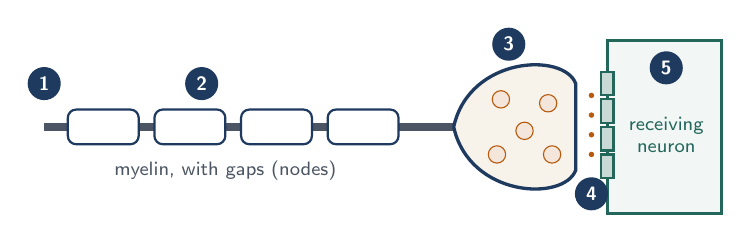
\begin{tikzpicture}[x=1cm,y=1cm]
    % axon with myelin
    \draw[kgrey,line width=3pt] (0,0) -- (5.2,0);
    \foreach \x in {0.3,1.4,2.5,3.6}{\draw[myel] (\x,-0.22) rectangle (\x+0.9,0.22);}
    \node[font=\scriptsize,text=kgrey] at (2.3,-0.55) {myelin, with gaps (nodes)};
    % terminal
    \draw[kprimary,very thick,fill=kpale] (5.2,0.0) .. controls (5.4,0.9) and (6.6,0.95) .. (6.75,0.55) -- (6.75,-0.55) .. controls (6.6,-0.95) and (5.4,-0.9) .. (5.2,0.0);
    \foreach \x/\y in {5.8/0.35,6.1/-0.05,5.75/-0.35,6.4/0.3,6.45/-0.35}{\node[ves] at (\x,\y) {};}
    % cleft and receiving cell
    \foreach \y in {-0.35,-0.1,0.15,0.4}{\node[tx] at (6.95,\y) {};}
    \draw[kgreen,very thick,fill=kgreen!6] (7.15,-1.1) -- (7.15,1.1) -- (8.6,1.1) -- (8.6,-1.1) -- cycle;
    \foreach \y in {-0.5,-0.15,0.2,0.55}{\node[rcp] at (7.15,\y) {};}
    \node[font=\scriptsize,text=kgreen,align=center] at (7.9,-0.1) {receiving\\neuron};
    % badges
    \node[badge] at (0.0,0.55) {1};
    \node[badge] at (2.0,0.55) {2};
    \node[badge] at (5.9,1.05) {3};
    \node[badge] at (6.95,-0.85) {4};
    \node[badge] at (7.9,0.75) {5};
  \end{tikzpicture}}
\newcommand{\relaylist}{%
  \begin{enumerate}\setlength{\itemsep}{3pt}
    \item \textbf{Along the axon:} each patch fires the next, like a fuse.
    \item \textbf{Myelin} makes the spike jump from gap to gap: much faster.
    \item \textbf{At the terminal:} \Ca\ rushes in; vesicles release transmitter.
    \item \textbf{Across the gap:} transmitter binds to \textbf{receptors}.
    \item \textbf{The receiving neuron} adds up its inputs and decides.
  \end{enumerate}}

% \saltpicture: bare versus myelinated conduction
\newcommand{\saltpicture}{%
  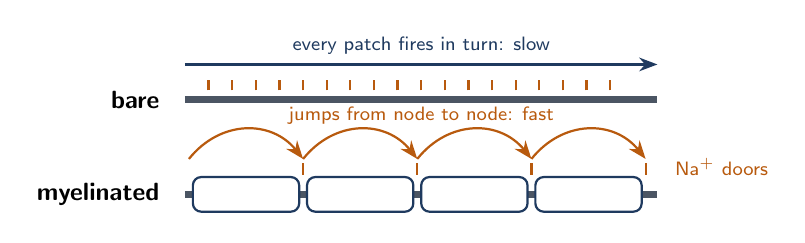
\begin{tikzpicture}[x=1cm,y=1cm]
    \node[font=\small\bfseries,anchor=east] at (-0.2,1.2) {bare};
    \draw[kgrey,line width=2.5pt] (0,1.2) -- (6,1.2);
    \foreach \x in {0.3,0.6,...,5.7}{\draw[cNa,thick] (\x,1.32) -- (\x,1.45);}
    \draw[-{Stealth},thick,kprimary] (0,1.65) -- (6,1.65) node[midway,above,font=\scriptsize]{every patch fires in turn: slow};
    \node[font=\small\bfseries,anchor=east] at (-0.2,0) {myelinated};
    \draw[kgrey,line width=2.5pt] (0,0) -- (6,0);
    \foreach \x in {0.1,1.55,3.0,4.45}{\draw[myel] (\x,-0.22) rectangle (\x+1.35,0.22);}
    \foreach \x in {1.5,2.95,4.4,5.85}{\draw[cNa,thick] (\x,0.25) -- (\x,0.4);}
    \foreach \a/\b in {0.05/1.5,1.5/2.95,2.95/4.4,4.4/5.85}{\draw[-{Stealth},thick,kaccent] (\a,0.45) .. controls (\a+0.4,0.95) and (\b-0.4,0.95) .. (\b,0.45);}
    \node[font=\scriptsize,text=kaccent] at (3,1.0) {jumps from node to node: fast};
    \node[font=\scriptsize,text=cNa,anchor=west] at (6.1,0.35) {Na$^{+}$ doors};
  \end{tikzpicture}}

% \synapsesteps: the six steps of a chemical synapse
\newcommand{\synapsesteps}{%
  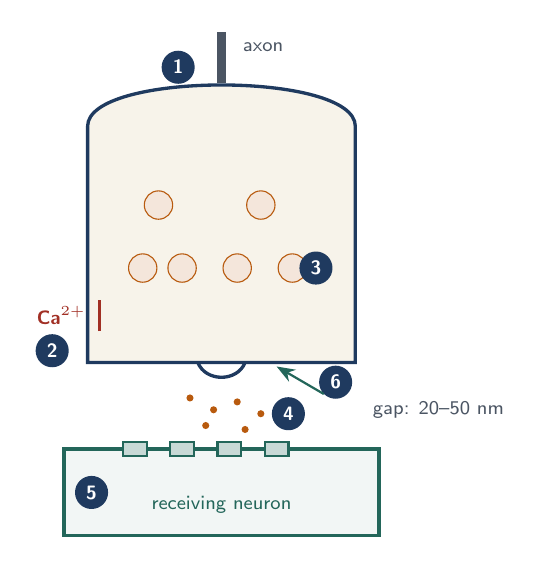
\begin{tikzpicture}[x=1cm,y=1cm]
    \draw[kprimary,very thick,fill=kpale] (0,0.2) -- (0,3.2) .. controls (0,3.9) and (3.4,3.9) .. (3.4,3.2) -- (3.4,0.2) -- cycle;
    \draw[kgrey,line width=3pt] (1.7,3.75) -- (1.7,4.4);
    \node[font=\scriptsize,text=kgrey,anchor=west] at (1.85,4.2) {axon};
    \foreach \x/\y in {0.7,1.2,1.9,2.6}{\node[ves,minimum size=0.36cm] at (\x,1.4) {};}
    \foreach \x in {0.9,2.2}{\node[ves,minimum size=0.36cm] at (\x,2.2) {};}
    \draw[cCa,very thick] (0.15,0.6) -- (0.15,1.0); \node[font=\scriptsize\bfseries,text=cCa,anchor=east] at (0.1,0.8) {Ca$^{2+}$};
    \draw[kprimary,very thick] (1.4,0.2) .. controls (1.5,-0.05) and (1.9,-0.05) .. (2.0,0.2);
    \foreach \x/\y in {1.3/-0.25,1.6/-0.4,1.9/-0.3,2.2/-0.45,1.5/-0.6,2.0/-0.65}{\node[tx,minimum size=0.09cm] at (\x,\y) {};}
    \draw[kgreen,very thick,fill=kgreen!6] (-0.3,-0.9) -- (3.7,-0.9) -- (3.7,-2.0) -- (-0.3,-2.0) -- cycle;
    \foreach \x in {0.6,1.2,1.8,2.4}{\node[rcp,minimum width=0.3cm,minimum height=0.18cm] at (\x,-0.9) {};}
    \node[font=\scriptsize,text=kgreen] at (1.7,-1.6) {receiving neuron};
    \node[font=\scriptsize,text=kgrey,anchor=west] at (3.5,-0.4) {gap: 20--50 nm};
    \node[badge] at (1.15,3.95) {1};
    \node[badge] at (-0.45,0.35) {2};
    \node[badge] at (2.9,1.4) {3};
    \node[badge] at (2.55,-0.45) {4};
    \node[badge] at (0.05,-1.45) {5};
    \node[badge] at (3.15,-0.05) {6};
    \draw[-{Stealth},kgreen,thick] (3.0,-0.2) -- (2.4,0.15);
  \end{tikzpicture}}
\newcommand{\synapselist}{%
  \begin{enumerate}\setlength{\itemsep}{2pt}
    \item A spike arrives at the terminal.
    \item \Ca\ doors open; \Ca\ rushes in.
    \item Vesicles fuse and release transmitter.
    \item Transmitter crosses the gap and binds to receptors.
    \item Receptor channels open: an \textbf{EPSP} or \textbf{IPSP}.
    \item Transmitter is cleared: reuptake or an enzyme.
  \end{enumerate}}
\newcommand{\lablink}{https://rakesh-sengupta.github.io/neural-signalling-labs/labs/relay-lab/}
\newcommand{\lablinkshown}{rakesh-sengupta.github.io/\\neural-signalling-labs/labs/relay-lab}
\newcommand{\Ca}{\textcolor{cCa}{\textbf{Ca$^{2+}$}}}
\newcommand{\Cl}{\textcolor{cCl}{\textbf{Cl$^{-}$}}}

\begin{document}
\RaggedRight

% ============================ PAGE 1 =================================
\pagehead{Sessions \sessnum: The relay}

\textbf{How to use this booklet.} Each Relay Lab part has its own page, with the time, who to work with, and the steps. You may always work alone. \textbf{Lost during class?} Page 2 has the whole session on one page; every term is on page 3.

\smallskip
{\renewcommand{\arraystretch}{1.3}
\begin{tabular}{@{}>{\raggedright\arraybackslash\bfseries}p{3.2cm}p{9.6cm}r@{}}
\toprule
Part & What we do & Time\\
\midrule
Opening & From one spike to the next neuron; open Relay Lab & 7 min\\
1 Along the axon & How a spike travels; myelin; MS (Lab Part 1, page 4) & 25 min\\
2 Across the gap & Sparks or soups? The chemical synapse; adding up (Lab Part 2, page 5) & 28 min\\
3 Keys and locks & Transmitters, receptors, drugs (Lab Part 3, page 6) & 22 min\\
Wrap-up & Today on one page, again; exit ticket & 8 min\\
\bottomrule
\end{tabular}}

\medskip
\begin{infobox}[title={Warm-up}]
You touch a hot pan. The message travels about a metre up your arm, then passes from one neuron to the next, several times. Where would you guess the time is lost: on the long trip \textbf{along the wires}, or at the \textbf{junctions} between them? My guess:
\lines{1}
\end{infobox}

\begin{infobox}[title={Exit ticket (end of class, 3 minutes)}]
1. Why does myelin make a spike faster?
\lines{1}
2. What does \Ca\ do at the axon terminal?
\lines{1}
3. One agonist: \blank[4cm] \quad One antagonist: \blank[4cm]
\end{infobox}

\smallskip
{\color{kgrey}\small \textbf{Next class: Quiz 2} (Sessions 7--12). Pages 2 and 8 of this booklet, and the ``today on one page'' sheets from Sessions 7 and 9, are good revision.}

% ============================ PAGE 2 =================================
\newpage
\pagehead{Today on one page}

From one neuron to the next, in five steps. If you lose the thread, find the number here.

\begin{center}
\resizebox{0.92\linewidth}{!}{\relaypicture}
\end{center}

\relaylist

\medskip
\begin{infobox}[title={Relay Lab (runs in any browser; nothing is saved or sent)}]
\begin{minipage}[c]{0.78\linewidth}
Open it on a laptop or phone and keep it beside the slides. Each part is locked until its slide (marked \textbf{RELAY LAB}) shows the password, so we move together. Part 1 is the race along the axon; Part 2 is adding up at the synapse; Part 3 is drugs at receptors.\\[4pt]
\textbf{\lablinkshown}
\end{minipage}\hfill
\begin{minipage}[c]{0.18\linewidth}\centering
\qrcode[height=2.3cm]{\lablink}
\end{minipage}
\end{infobox}

% ============================ PAGE 3 =================================
\newpage
\pagehead{Word list}

Keep this beside you during the lab.

{\renewcommand{\arraystretch}{1.22}\small
\begin{tabular}{@{}>{\bfseries}p{4.4cm}p{12cm}@{}}
\toprule
conduction velocity & how fast a spike travels along an axon, in metres per second (m/s)\\
myelin & fatty wrapping around an axon, made by glial cells; it stops current leaking out\\
node of Ranvier & a short gap in the myelin, packed with \Na\ doors, where the spike is rebuilt\\
saltatory conduction & the spike ``jumping'' from node to node (Latin \emph{saltare}, to jump)\\
multiple sclerosis (MS) & a disease in which the immune system damages myelin in the brain and spinal cord\\
synapse & the junction where one neuron passes a signal to another\\
electrical synapse & a gap junction: ions flow straight through from cell to cell (gap about 3 nm)\\
chemical synapse & a synapse where a chemical crosses a gap of 20--50 nm\\
presynaptic / postsynaptic & the sending side / the receiving side of a synapse\\
vesicle & a tiny bubble (about 50 nm) filled with transmitter\\
exocytosis & a vesicle fusing with the membrane and releasing its contents\\
neurotransmitter & the chemical messenger released at a synapse\\
receptor & a protein that the transmitter binds to, like a key in a lock\\
EPSP / IPSP & a small push towards threshold (excitatory) / away from it (inhibitory)\\
summation & adding up inputs: \emph{spatial} (several at once) or \emph{temporal} (one, repeated fast)\\
ion-channel receptor & a receptor that is itself a door: fast (milliseconds)\\
G-protein receptor & a receptor that works through messengers inside the cell: slower, longer, amplified\\
agonist / antagonist & a drug that switches a receptor on / one that blocks it\\
reuptake & transmitter pumped back into the terminal, ending the signal\\
\bottomrule
\end{tabular}}

% ============================ PAGE 4 =================================
\newpage
\pagehead{Relay Lab, Part 1: the race}
\actinfo{8 minutes}{alone or in pairs}{a laptop or phone}

\begin{stepsbox}
\cb Open Relay Lab (page 2) and press \textbf{Continue}. Type the password from the slide and press \textbf{Unlock}.\\[3pt]
\cb Choose an axon and press \textbf{Send a spike}. It races 10 cm between two electrodes.\\[3pt]
\cb Race all four axons in the table below.\\[3pt]
\cb Type each speed into the lab and press \textbf{Check}.
\end{stepsbox}

\textbf{Predict first.} Which will be faster: the squid giant axon (500 \textmu m thick, bare) or a 12 \textmu m myelinated axon from your arm?\quad \cb squid \quad \cb myelinated

\medskip
{\renewcommand{\arraystretch}{1.9}
\begin{tabular}{@{}|p{6.6cm}|p{3cm}|p{2.6cm}|p{3cm}|@{}}
\hline
\textbf{Axon} & \textbf{Time for 10 cm} & \textbf{Speed} & \textbf{Time for 1 m}\\ \hline
1 \textmu m, bare (like a pain fibre) & \hfill ms & \hfill m/s & \hfill ms\\ \hline
12 \textmu m, myelinated & \hfill ms & \hfill m/s & \hfill ms\\ \hline
squid giant axon, 500 \textmu m, bare & \hfill ms & \hfill m/s & \hfill ms\\ \hline
12 \textmu m, damaged myelin patch & \hfill ms & \hfill m/s & \hfill ms\\ \hline
\end{tabular}}

\smallskip
{\small\color{kgrey}Time for 1 m $=$ time for 10 cm $\times$ 10. A metre is roughly from your toe to your spinal cord.}

\medskip
\textbf{1.} The squid axon is about 40 times thicker. Why does the thin myelinated axon still win?
\lines{2}
\textbf{2.} In MS, patches of myelin are damaged. Using your last row, why might someone with MS see, feel or move more slowly?
\lines{2}

% ============================ PAGE 5 =================================
\newpage
\pagehead{Relay Lab, Part 2: adding up}
\actinfo{8 minutes}{alone or in pairs}{a laptop or phone}

\begin{stepsbox}
\cb Type the password from the slide and press \textbf{Unlock}. Put the six steps of a chemical synapse in order (write them below too).\\[3pt]
\cb Fire input A alone, then A + B, then A + B + C. Then add D (inhibitory).\\[3pt]
\cb Fire A three times; find the \textbf{longest} gap that still makes a spike.\\[3pt]
\cb Type your three numbers into the lab and press \textbf{Check}.
\end{stepsbox}

\textbf{The six steps, in order} (from ``a spike arrives'' to ``transmitter is cleared''):\\[2pt]
{\renewcommand{\arraystretch}{1.6}
\begin{tabular}{@{}r p{7cm} r p{7cm}@{}}
1 & \blank[6.6cm] & 4 & \blank[6.6cm]\\
2 & \blank[6.6cm] & 5 & \blank[6.6cm]\\
3 & \blank[6.6cm] & 6 & \blank[6.6cm]\\
\end{tabular}}

\medskip
{\renewcommand{\arraystretch}{1.75}
\begin{tabular}{@{}|p{6.4cm}|p{4.2cm}|p{4.2cm}|@{}}
\hline
\textbf{What you fired} & \textbf{Highest rise above rest} & \textbf{Spike?}\\ \hline
A alone & & \cb yes \quad \cb no\\ \hline
A + B & & \cb yes \quad \cb no\\ \hline
A + B + C & & \cb yes \quad \cb no\\ \hline
A + B + C + D & & \cb yes \quad \cb no\\ \hline
\end{tabular}}

\smallskip
Rise from A alone (above $-65$ mV): \blank[2.2cm] mV \qquad Inputs needed together: \blank[1.6cm]\\[8pt]
Longest gap that still fires, A three times: \blank[2.2cm] ms

\medskip
\textbf{1.} Spatial or temporal summation? \quad A + B + C: \blank[2.4cm] \quad A three times: \blank[2.4cm]

\medskip
\textbf{2.} At a muscle, one spike always fires the muscle. Why is it useful that a brain neuron needs several inputs?
\lines{2}

% ============================ PAGE 6 =================================
\newpage
\pagehead{Relay Lab, Part 3: keys and locks}
\actinfo{8 minutes}{alone or in pairs}{a laptop or phone}

\begin{stepsbox}
\cb Type the password from the slide and press \textbf{Unlock}. Pick a synapse and press \textbf{Release transmitter} with no drug.\\[3pt]
\cb Try the \textbf{agonist}, the \textbf{antagonist} and the \textbf{clearance blocker}. Watch both panels.\\[3pt]
\cb Do this for the muscle (ion channel) and for one G-protein synapse. Fill in the table.
\end{stepsbox}

Write the peak (no drug $=$ 100), and how long the response lasts. Is it bigger or smaller, longer or shorter?

{\renewcommand{\arraystretch}{1.85}
\begin{tabular}{@{}|p{4.1cm}|p{5.6cm}|p{5.6cm}|@{}}
\hline
\textbf{Drug} & \textbf{ACh at a muscle (ion channel)} & \textbf{G-protein synapse: \blank[1.6cm]}\\ \hline
none & 100, lasts \blank[1.2cm] ms & 100, lasts \blank[1.2cm] ms\\ \hline
agonist & & \\ \hline
antagonist & & \\ \hline
clearance blocker & & \\ \hline
\end{tabular}}

\medskip
\textbf{Match each real drug to what it does.} Write \textbf{Ag} (agonist), \textbf{An} (antagonist) or \textbf{B} (blocks clearance).

{\renewcommand{\arraystretch}{1.55}
\begin{tabular}{@{}p{0.9cm}p{7cm}p{0.9cm}p{7cm}@{}}
\blank[0.7cm] & \textbf{Curare}: arrow-tip poison; paralyses muscles & \blank[0.7cm] & \textbf{Nicotine}: switches on muscle ACh receptors\\
\blank[0.7cm] & \textbf{Caffeine}: stops adenosine making you drowsy & \blank[0.7cm] & \textbf{Fluoxetine (Prozac)}: stops serotonin reuptake\\
\blank[0.7cm] & \textbf{Atropine}: eye drops that widen the pupil & \blank[0.7cm] & \textbf{Nerve gas}: stops the enzyme that breaks down ACh\\
\end{tabular}}

\medskip
\textbf{Think.} Fluoxetine blocks reuptake within hours, yet its effect on mood takes weeks. What does that suggest about how it works?
\lines{1}

% ============================ PAGE 7 =================================
\newpage
\pagehead{Study cards}
\small

\begin{studycard}[title={Soups or sparks? Eccles and Popper (1940s--1951)}]
Did neurons talk with electricity (``sparks'') or chemicals (``soups'')? John Eccles backed sparks. The philosopher Karl Popper told him a good theory should be stated so it could be proved wrong, and that he should try to refute his own. In 1951 Eccles's own recordings did just that: inhibition needed a chemical. He switched sides, and shared the 1963 Nobel Prize. Electrical synapses do exist, but most synapses are chemical \emph{(Valenstein, 2005; Brock, Coombs \& Eccles, 1952)}.
\end{studycard}

\begin{studycard}[title={Bernard Katz: transmitter comes in packets (1950s)}]
At the frog muscle, Katz saw tiny responses all of the same size: one vesicle each, a \textbf{quantum}. A spike at a muscle releases about 200 vesicles: a large, safe response. In the brain, one synapse may release a single vesicle, giving a push of a fraction of a millivolt \emph{(Bear, Ch.~5)}.
\end{studycard}

\begin{studycard}[title={Myelin in trouble: MS and Guillain--Barré}]
In \textbf{multiple sclerosis}, the immune system attacks myelin in the brain and spinal cord; signals slow or fail. A checkerboard pattern on a screen can show the slowing in the visual pathway. In \textbf{Guillain--Barré syndrome}, it attacks myelin in the nerves of the body, weakening the muscles \emph{(Bear, Box 4.5)}.
\end{studycard}

\begin{studycard}[title={Poisons that taught us the synapse}]
\textbf{Botulinum toxin} (spoiled canned food) stops ACh release. \textbf{Black widow venom} makes terminals dump all their ACh. \textbf{$\alpha$-Bungarotoxin} (a snake venom) and \textbf{curare} (an arrow poison) block the ACh receptor. Each stops a different step \emph{(Bear, Box 5.5)}.
\end{studycard}

\begin{studycard}[title={Startle disease and strychnine}]
In \textbf{hyperekplexia}, a faulty glycine receptor weakens inhibition, so a sudden noise can make a person go stiff and fall. The poison \textbf{strychnine} blocks the same receptor, causing convulsions. Inhibition matters as much as excitation \emph{(Bear, Box 5.6)}.
\end{studycard}

\begin{studycard}[title={Snyder and Pert: the brain's own morphine (1973)}]
Candace Pert and Solomon Snyder labelled opiate drugs with radioactivity and found they stuck to specific sites: \textbf{opiate receptors}. Why would the brain have receptors for a poppy drug? Because it makes its own: the \textbf{enkephalins} were found soon after \emph{(Pert \& Snyder, 1973; Bear, Ch.~6)}.
\end{studycard}
\normalsize

% ============================ PAGE 8 =================================
\newpage
\pagehead{Transmitter cheat sheet}

\textbf{Three families} (almost every transmitter is made from amino acids):

{\renewcommand{\arraystretch}{1.35}
\begin{tabular}{@{}>{\bfseries}p{3.4cm}p{6.4cm}p{6.4cm}@{}}
\toprule
Family & Examples & Notes\\
\midrule
Amino acids & glutamate, GABA, glycine & fast; glutamate usually excites, GABA and glycine usually inhibit\\
Amines & acetylcholine (ACh), dopamine, noradrenaline, serotonin, histamine & ACh moves your muscles; the others set mood, attention, sleep\\
Peptides & enkephalins, substance P & short chains of amino acids; slow, long-lasting\\
\bottomrule
\end{tabular}}

\medskip
\textbf{One key, many locks} (from Bear, Table 6.1):

{\renewcommand{\arraystretch}{1.3}
\begin{tabular}{@{}>{\bfseries}p{3.0cm}p{4.2cm}p{4.1cm}p{4.3cm}@{}}
\toprule
Transmitter & Receptor & Agonist & Antagonist\\
\midrule
ACh & nicotinic (muscle) & nicotine & curare\\
ACh & muscarinic (heart) & muscarine & atropine\\
Glutamate & AMPA, NMDA & AMPA, NMDA & CNQX, AP5\\
GABA & GABA$_\mathrm{A}$ & muscimol & bicuculline\\
Adenosine & A type & adenosine & caffeine\\
\bottomrule
\end{tabular}}

\medskip
\textbf{Two kinds of lock:}

{\renewcommand{\arraystretch}{1.35}
\begin{tabular}{@{}>{\bfseries}p{3.4cm}p{6.4cm}p{6.4cm}@{}}
\toprule
 & Ion-channel receptor & G-protein receptor\\
\midrule
How it works & the receptor is itself a door; ions flow at once & the receptor wakes up G-proteins inside the cell; they act on doors or enzymes\\
Speed & milliseconds & hundreds of milliseconds to seconds\\
Amplification & none & one receptor can activate 10--20 G-proteins\\
Example & ACh at a muscle & ACh at the heart; most serotonin receptors\\
\bottomrule
\end{tabular}}

% ============================ PAGE 9 =================================
\newpage
\pagehead{Answers (check after class)}

\textbf{Warm-up.} The trip along a fast myelinated axon is quick (a metre in about 14 ms). Much of the time in a reaction goes on synapses and on neurons adding up their inputs.

\textbf{Part 1.} 1 \textmu m bare: 100 ms, \textbf{1 m/s}, 1000 ms for 1 m. 12 \textmu m myelinated: 1.4 ms, \textbf{72 m/s}, 14 ms. Squid: 4.5 ms, \textbf{22 m/s}, 45 ms. Damaged myelin: 9.6 ms, \textbf{10 m/s}, 96 ms. (1) Myelin stops current leaking out, so the spike only has to be rebuilt at the nodes and jumps between them; thickness alone is a costly way to speed up. (2) Where myelin is damaged, the spike crawls (or fails), so signals in vision, touch and movement arrive late or not at all.

\textbf{Part 2.} Steps: spike arrives; \Ca\ doors open and \Ca\ rushes in; vesicles fuse and release transmitter; transmitter crosses and binds to receptors; receptor channels open (EPSP or IPSP); transmitter is cleared. Highest rise: A alone about \textbf{7 mV} (threshold is 15 mV above rest), no spike; A + B about 13.5 mV, no spike; A + B + C: spike; A + B + C + D about 12.4 mV, no spike. Inputs needed: \textbf{3}. Longest gap: \textbf{7 ms}. (1) Spatial; temporal. (2) A brain neuron weighs many inputs and decides; a single noisy input does not set it off.

\textbf{Part 3.} Muscle: none 100 (about 8 ms); agonist already on before release, peak about 150; antagonist about 15; blocker about 210, lasting about 22 ms. Serotonin: none 100 (about 320 ms); agonist peak about 160; antagonist 15; blocker about 290, lasting about 590 ms. Heart (muscarinic): none 100 (about 270 ms); agonist about 165; antagonist 15; blocker about 305. Matching: curare An, nicotine Ag, caffeine An, fluoxetine B, atropine An, nerve gas B. Think: blocking reuptake cannot be the whole story. The slow effect suggests the brain itself changes over weeks in response to the extra serotonin; exactly how is still being studied.

\textbf{Exit ticket.} (1) The spike only has to be rebuilt at the nodes and jumps between them. (2) \Ca\ rushes in and makes vesicles fuse and release transmitter. (3) For example, agonist: nicotine; antagonist: curare, atropine or caffeine.

% ============================ PAGE 10 ================================
\newpage
\pagehead{Sources}
\small
\begin{itemize}[leftmargin=1.2em,itemsep=2pt]
\item Bear, M.\,F., Connors, B.\,W., \& Paradiso, M.\,A.\ (2016). \emph{Neuroscience: Exploring the Brain} (4th ed.), Chapters 4, 5 and 6 (Boxes 4.5, 5.5, 5.6; Table 6.1).
\item Borck, C.\ (2017). Soups and sparks revisited. \emph{Nuncius} 32, 286--329.
\item Brock, L.\,G., Coombs, J.\,S., \& Eccles, J.\,C.\ (1952). The recording of potentials from motoneurones with an intracellular electrode. \emph{Journal of Physiology} 117, 431--460.
\item de Leeuw, J.\,R.\ (2015). jsPsych: a JavaScript library for creating behavioral experiments in a web browser. \emph{Behavior Research Methods} 47, 1--12.
\item Hursh, J.\,B.\ (1939). Conduction velocity and diameter of nerve fibers. \emph{American Journal of Physiology} 127, 131--139.
\item Pert, C.\,B., \& Snyder, S.\,H.\ (1973). Opiate receptor: demonstration in nervous tissue. \emph{Science} 179, 1011--1014.
\item Purves, D., et al.\ (Eds.) \emph{Neuroscience}. Sinauer. Fibre classes and conduction velocities.
\item Valenstein, E.\,S.\ (2005). \emph{The War of the Soups and the Sparks}. Columbia University Press.
\item Relay Lab, Part 1: conduction speeds from rules of thumb fitted to real nerves (myelinated: about 6 m/s per \textmu m of diameter, after Hursh 1939; bare: about $\sqrt{d}$ m/s), not a simulation. The damaged patch covers 3 of the 10 cm.
\item Relay Lab, Part 2: a leaky integrate-and-fire neuron with conductance-based synapses (membrane time constant 15 ms; rest $-65$ mV; threshold $-50$ mV).
\item Relay Lab, Part 3: simplified receptor kinetics in arbitrary units, scaled so that no drug $=$ 100. The directions of the effects are what matter, not the exact numbers.
\end{itemize}
\end{document}
